\documentclass[a4paper,10.0pt,twoside]{npr}

\usepackage{multicol,graphicx,lastpage,footmisc,fancyhdr,paralist,
tabularx,array,booktabs,caption,multirow,upgreek,mathrsfs,gensymb,color}
\usepackage[fancyhdr,space,fntef,fontset=ubuntu]{ctex}
\usepackage{amssymb,bm,mathrsfs,bbm,amscd}
\usepackage{flushend,cuted}
\usepackage{refcount}
\usepackage{savesym}
\usepackage{textcomp}
\usepackage[tbtags]{amsmath}  %
\savesymbol{iint}
\usepackage{amstext} %数学宏包文本命令
\usepackage{balance} %版心底部对齐

\flushbottom      %版心底部对齐
\setcounter{section}{0}
\begin{document}
%\begin{CJK*}{GBK}{\song}{\wuhao}{\rm}

%___________________________________________________________________________________
\def\rd{{\rm d}}

\newcommand{\RM}{\ensuremath{\mathrm}}   %正体 既可用于文本模式也可用于数学模式
\newcommand{\dif}{\mathrm{d}}  %直立体d
\newcommand{\me}{\mathrm{e}}  %直立体e
\newcommand{\mi}{\mathrm{i}}  %直立体i
\newcommand{\mj}{\mathrm{j}}  %直立体j
\newcommand{\afrac}[2]{\dfrac{\,#1\,}{\,#2\,}}  %略长分数线
\newcommand{\nn}{\nonumber}  %公式无编号
\newcommand{\nt}{\noindent}
\newcommand{\OO}{~\text{。}}
\newcommand{\PP}{~\text{,}}
\newcommand{\OP}{~\text{;}}
\newcommand{\LT}{\left}
\newcommand{\RT}{\right}

%___________________________________________________________________________________

\balance
\fancypagestyle{myfoot}
{%
\fancyhf{}
\fancyhead[c]{\wuhao\song 粒~子~物~理~与~原~子~核~物~理~专~题~实~验}
\renewcommand{\headrule}{\vskip 2pt
\hrule height0.4pt width\headwidth \vskip1pt
\hrule height0.4pt width\headwidth \vskip-1.8pt}
}%
\thispagestyle{myfoot}

%%%%%%%%%%%%%%%%%%%%%%%%%%%%%%%%%%%%%%%%%%%%%%%%%%%%%
%    奇偶页眉
%%%%%%%%%%%%%%%%%%%%%%%%%%%%%%%%%%%%%%%%%%%%%%%%%%%%%
\pagestyle{fancy}
\fancyhead{}
\fancyhead[ce]{\xiaowu\song \hspace{0.5em}粒~子~物~理~与~原~子~核~物~理~专~题~实~验}
%\fancyhead[ro,le]{\xiaowuhao \hspace{0.5em}\textbf{\textperiodcentered}\;\thepage\;\textbf{\textperiodcentered}\hspace{0.5em}}
%\fancyhead[ce]{\xiaowu\song 粒~子~物~理~与~原~子~核~物~理~专~题~实~验}
%\fancyhead[re]{\xiaowu\song \hspace{0.5em}第\;31\;卷\hspace{0.5em}}
\fancyfoot[ce,co]{}
\renewcommand{\headrule}{\vskip 2pt
\hrule height0.4pt width\headwidth}


\setcounter{page}{001}%
\fancyhead[co]{\xiaowuhao\song  乔颢:半导体$\alpha$谱仪和$\alpha$粒子的能量损失}    %奇页页眉
\begin{center}
\title{%
\xiaoerhao \bf  %章标题为两行时改为 \exiaoer
半导体$\alpha$谱仪和$\alpha$粒子的能量损失\\[-5mm]}
\maketitle
\large \fs
乔颢$^{^1}$\\[2mm]

\xiaowu \song
1. 北京大学物理学院,海淀区 北京 100871;\\[4mm]

 
\footnotetext[0]{{\bf 作者简介:}~~\begin{minipage}[t][4.2mm]{149mm}\song
乔颢,E-mail: i@catofes.com
\end{minipage} }
%\footnotetext[0]{{\bf 通信作者:}\song ~~E-mail: xxx@xxx.xxx }%通信作者为第一作者时不要此项

\parbox{158mm} {
\zywu{\bf 摘要:}~~\fs
摘要中应介绍工作目的、方法、结果和最终结论,
摘要应为独立的小短文,以第三人称撰写, 避免使用"本文"、"作者"等词汇。中文摘要300字左右。

{\bf 关键词:}~~\fs 半导体$\alpha$谱仪, $\alpha$粒子, $^{241}Am$(2-4个) \\
{\bf PACS:}~~\song 与主题一致。}
\end{center}
%%%%6.正文
\vspace{5mm}
%%%%6.正文
\setcounter{section}{0}
\begin{multicols}{2}
%----------------
%____________________________________________________________________________
%%%%以上请不要改动%%%%%%%%%%%%%%%%%%%%%%%%%%%%%%%%%%%%%%%%%%%%

\section{引言}    %1
\vspace*{-1mm}
\song\wuhao
$\alpha$粒子是核物理实验中最常接触的一种粒子,研究其与物质的相互作用有助于理解高能粒子与物质的基本相互作用的形式及影响。天然$\alpha$的能量相对较低,大约在3-8MeV,在这个能量范围内,$\alpha$粒子一般通过与核外电子的相互作用而沉积能量。通过研究$\alpha$粒子经过物质时能量损失的规律,还能够测量薄膜的厚度,从而提供了一种较为精确的测量材料厚的方法。

半导体$\alpha$谱仪一般是有金硅面垒探测器和其后续的电子学电路所组成的。$\alpha$粒子入射入探测器的灵敏区内,与物质作用产生电子、空穴对,在反向电压的作用下被探测器收集,经过后续电路放大得到探测信号。金硅面磊半导体$\alpha$谱仪具有能量分辨率高,线性范围宽,脉冲上升时间快,价格便宜等优势,所以对于$\alpha$粒子而言他是一个良好且常用的探测器。

\section{实验}
金硅面垒半导体$\alpha$谱仪是一种优良的测量$\alpha$粒子以及其他带电重离子的装置。其组成结构如图1所示,当带电粒子进入半导体的PN结区域,也就是探测器的灵敏区后,其损失能量产生电子孔穴对。而产生电子孔穴对的能量$\omega$则只与材料有关。所以当入射粒子将能量全部沉积在灵敏体积时,其产生的总电荷量就为$\frac{E}{\omega} e$。 同时通过PN结所加的反向电压进行收集,汇集到两极形成电荷脉冲。

\begin{center}
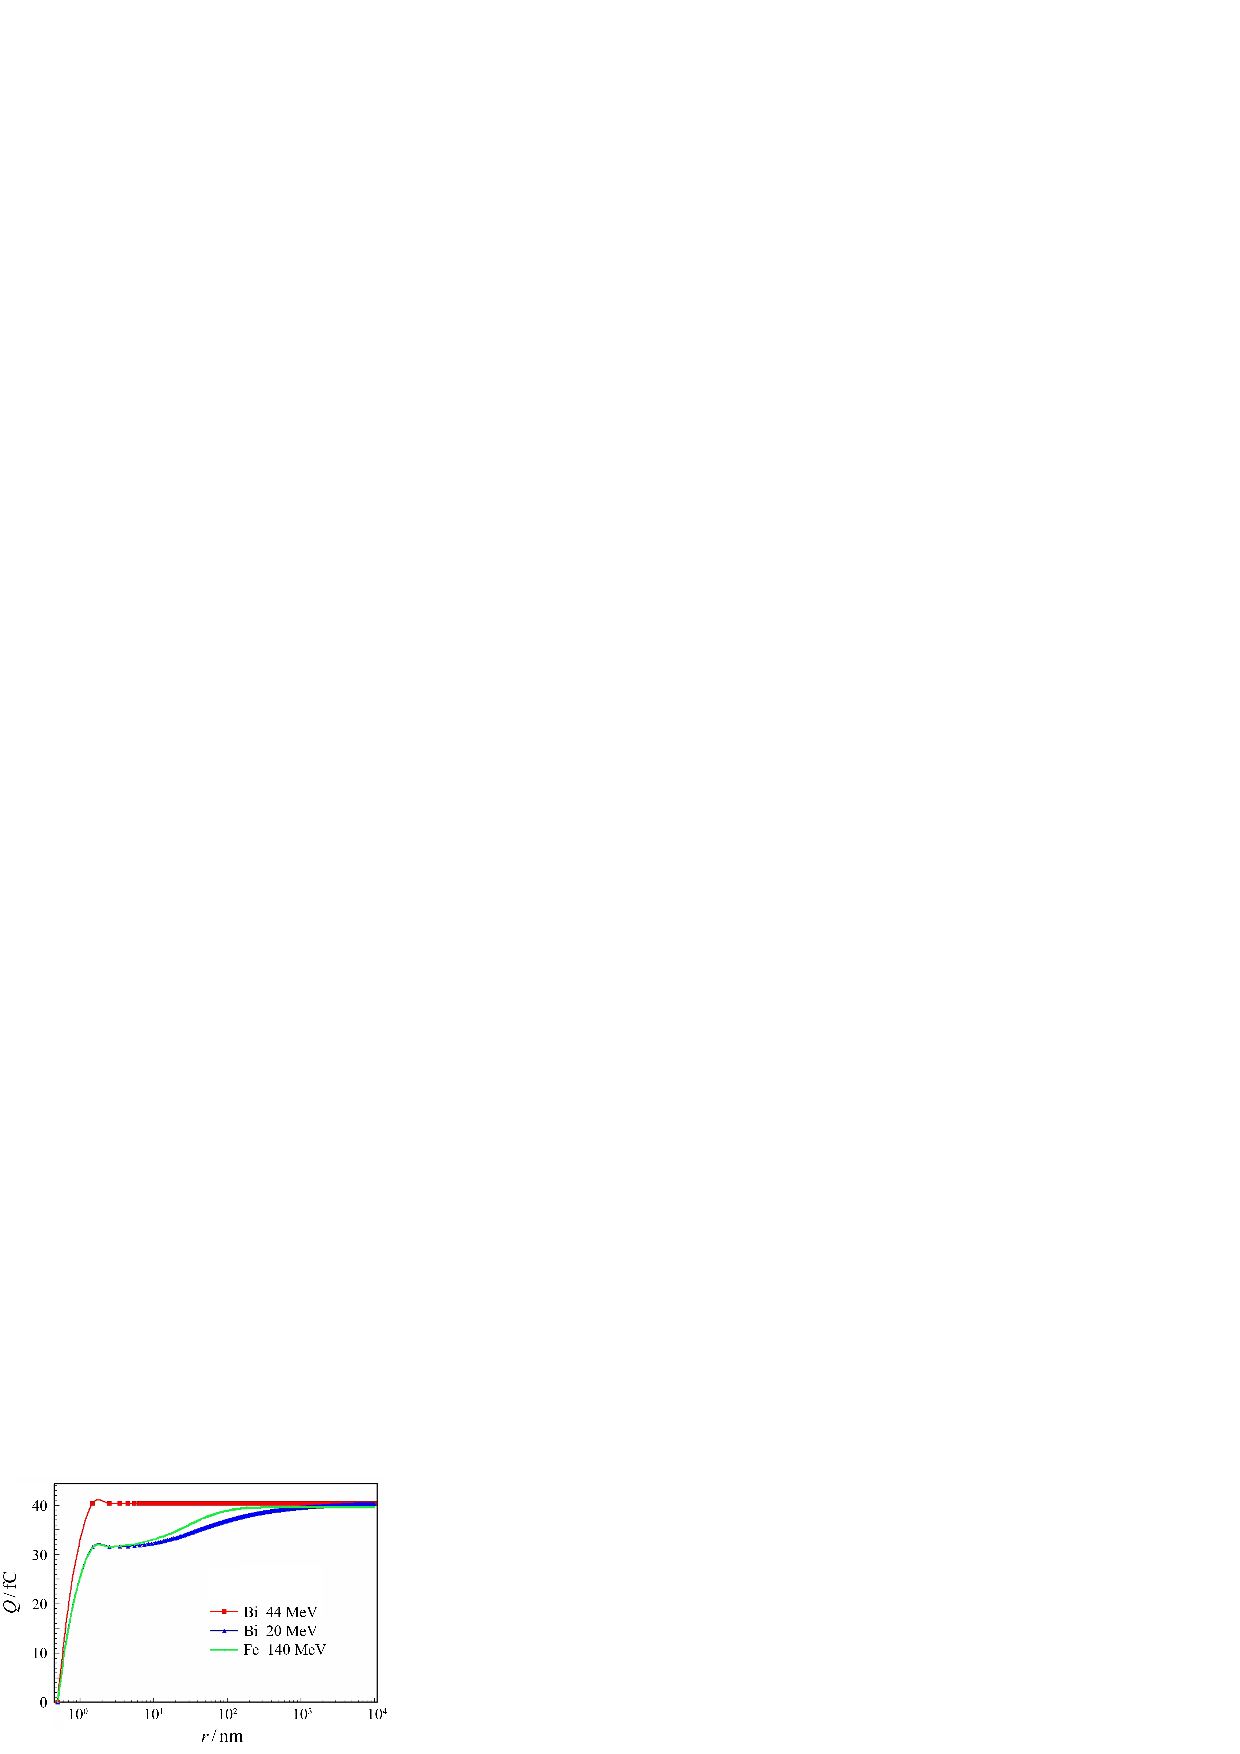
\includegraphics[width=0.4\textwidth]{tu1.png}\\
\xiaowu\song 图~1\begin{minipage}[t]{75mm} \quad 金硅面垒半导体探测器装置示意图。前级电荷放大器的输出信号经过线性放大器放大即可输入至多道等分析仪器进行分析。\\[-1mm]\wuhao
\end{minipage}
\end{center}

但是因为半导体结电容$C_d$的存在,金硅面垒探测器直接输出的脉冲信号幅度是$Q/C_d$,这样就会因为探测器所加偏压的微小变化而造成输出信号的幅度。从而导致探测结果的不精确,所以在探测器后面一般会接上一级前级放大器。在合理的选择前级放大器的电路,放大倍数以及反馈电容后,可以得到放大器输出的电压为
\begin{equation}\label{eq:1}
	V_0 =\frac{Q}{C_f}
\end{equation}
其中$C_f$是反馈电容的大小。具体的等效电路见图2。

\begin{center}
   \def\svgwidth{0.4\textwidth}
   \input{fangdaqi.eps_tex}
\\
\xiaowu\song 图~2\begin{minipage}[t]{75mm} \quad 探测器的等效电路以及前置放大器的电路图。图中$C_d$即为半导体探测器的等效结电容,$C'$为接线电缆等电容,经过前级放大器K倍放大后,若$KC_f>>C_d+C_1$,则最终输出电压满足上述公式\ref{eq:1}中的结果。\\[-1mm]\wuhao
\end{minipage}
\end{center}

通过使用半导体$\alpha$谱仪,我们可以非常方便的得到$\alpha$粒子的能谱,从而能够对$\alpha$粒子与物质的相互作用进行深一步的研究。$\alpha$粒子一般与物质的核外电子发生相互作用,其与电子碰撞使得原子电离,从而损失能量。又因为$\alpha$粒子的质量远远大于电子的质量,因而每次碰撞所转移给电子的能量有一个最大值,同时粒子的方向基本不发生改变。带电粒子在吸收体内单位长度损失的能量被称作线性阻止本领S。将S除以吸收体单位体积内的原子数N,得到物质的阻止截面$\Sigma_e$。 对于$\alpha$离子的阻止截面,可以得到一个经验公式:
\begin{equation}
	\Sigma_e=\frac{A_1 EA_2 \{ \frac{A_3}{E/1000}\ln[1+\frac{A_4}{E/1000}+\frac{A_5 E}{E/1000}]\}}{A_1 EA_2+\frac{A_3}{E/1000}\ln[1+\frac{A_4}{E/1000}+\frac{A_5 E}{E/1000}]}
\end{equation}
其中$A_1$到$A_5$是与材料有关的常数。

在知道阻止截面和能量的关系,以及$\alpha$粒子穿过物质后所损失的能量,我们就可以很方便的得到物质的厚度,这也就是通过$\alpha$粒子测量物质厚度方法的原理。



\section{实验结果和讨论}
此部分是实验报告的主体, 应占报告篇幅的一半以上。

依自己意愿, 实验结果和对结果的分析讨论既可分为两节也可合在一节。

实验结果应尽量以图表的形式给出。 每一个图表都应该是完整的, 即阅读图表时可以不必依赖正文。

对于预料之外的实验结果, 必须首先小心证明其可靠性.读者只有在相信你的实验结果时才愿意花时间看你的分析。

必须用文字归纳整理出正式的实验结果或结论.可信的实验结果是课程报告最重要的内容.作为一个实验物理工作者, 分析解释出错并不丢脸, 实验结果不被采信则是致命的.
教学实验的结论往往是预先知道的. 所以, 教师更关心的是你的说理过程. 一般说来, 单由课内实验的结果不足以能得到明确的结论. 此时, 你可以引用他人的研究结果来帮助帮助自己的论证, 但必须注明出处。

确实不能得到明确结论时, 可以给出几种可能结论并指出可以再做哪些实验来帮助作进一步的判断。

总之, 分析讨论部分要做到: 论据要valid, 论证要reasonable, 结论要convincing.


3.1 公式例子

单行公式:
\begin{equation}
f(r,p)=\frac{1}{N}\sum_{i=1}^{\tilde{N}N}\delta(r-r_{\RM{i}})\delta(p-p_{\RM{i}}) ~,%(1)
\end{equation}

多行公式,每行居中:
\begin{gather}  %多行公式,每行居中
\frac{\partial f}{\partial t}+\upsilon \cdot {{\nabla }_{r}}f-{{\nabla }_{r}}U\cdot {{\nabla }_{p}}f=\nonumber\\
 -\frac{1}{(2\uppi )^3}{\RM{d}^3}p'_{2}\RM{d}^{3}p{'}_{2}\RM{d}
 \Omega \frac{\RM{d}\sigma }{\RM{d}\Omega }v_{12}\times \nonumber\\
\{[f\/f_{2}(1-f'_{1})(1-f'_{2})]~,  %(2)
\end{gather}
多行公式,等号对齐:
\begin{align}  %多行公式,等号对齐
E_{sym}=&E_{sym}(\rho_0)+\frac{L(\rho_0)}{3}\left(\frac{\rho-\rho_0}{\rho_0}\right)+ \nonumber \\
& \frac{K_{sym}(\rho_0)}{18}\left(\frac{\rho-\rho_0}{\rho_0}\right)^2~\text{。}
  %(3)
\end{align}

3.2 图表要求
%\song\wuhao

图形要求:  彩色、黑白图形均可。

(1)~~在文稿中按插图出现的先后次序顺序编号,并在正文相应位置处插入图片。

(2)~~本刊为黑白印刷,彩图可在网刊中显示,如
需要请在图题中注明\,(在线彩图(中文稿),color online(英文稿))。图中的数据线可用黑色或彩色颜色(深色:红、兰、深绿等)来区别,不要用
浅色(黄、浅黄、浅粉等)或明暗来区分线条、符号和区域,建议使用不同方式来区别,比如:

1)~~线条:------,-- -- --,……,--$\cdot$--$\cdot$--,---$\bullet$---,---$\circ$---,---$\blacktriangle$---,---$
\blacksquare$---,---$\square$--- 等;

2)~~符号:$\triangleright$,$\bullet$,$\vartriangle$,$\blacktriangle$,$ \blacktriangledown$,$\blacktriangleleft$,$\blacktriangleright $ 等;

3)~~区域:黑、白、网格等。

(3)~~由于本刊为双栏排版,所以文章中图形通常不超过\,7.5cm\,(最好\,6.6cm\,左
右,方框净尺寸\,5.5cm),复杂图形不超过\,15cm。

(4)~~\textbf{图中的字母及数字用\,Times New Roman\,字体,中文用宋体,分辨率为\,600 dpi,字符大小用小\,5(9 Pt)号及\,6\,号\,(7.5 Pt)。}


(5)~~\textbf{图的横纵坐标刻度线应标在内侧},横纵坐标需标明相应的变量
和单位,使用“变量名称\,/\,单位”形式标记(如: $E$\,/\,keV)。


(6)~~{图中出现的物理量名称和符号须与正文一致
并在正文中有相关说明
和解释,若是中文稿,图中出现的英文描述内容请改用中文表达\,(非物理量名称),并
与文中的说明文字一致。}


(7)~~{所有插图需另提供\,1\,份画图软件的源数据文件,比
如\,Origin\,的\,opj}(word\,文件可直接将\,opj\,插入\,word\,文档中),{或提供高
分辨原图,或含图的文献\,pdf\,文件,以备修图制版。所有插图打包压缩
为一个文件上传或发到邮箱,并注明稿号。}


图形具体要求请参看 http://www.npr.ac.cn 。图例如下所示:

单栏图:
\begin{center}
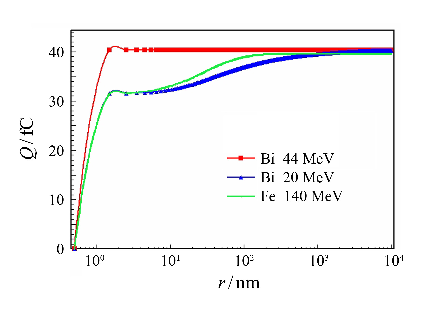
\includegraphics{tu1.eps}\\
\xiaowu\song 图~1\begin{minipage}[t]{75mm} \quad (在线彩图)\,不同种类、能量的离子沉积的电荷量沿径向的变化关系\\[-1mm]\wuhao
\end{minipage}
\end{center}
通栏图:
\end{multicols}

\begin{center}
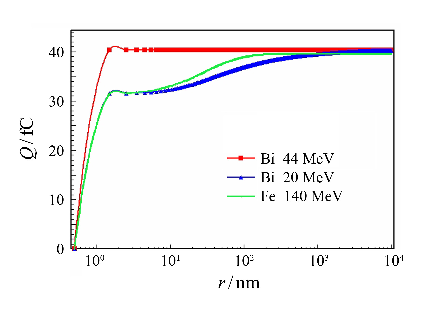
\includegraphics{tu1.eps}\\
\xiaowu\song  图~2\begin{minipage}[t]{160mm} \quad ImQMD05模型计算的电荷多重数分布与实验数据比较\\
\footnotesize
(a)\,入射能量为\,50\,MeV/u,中心碰撞条件
下\,Xe+Sn\,反应出射产物的电荷分布;(b)\,入射能量为\,35\,MeV/u\,中心碰撞条件下\,Ca+Ca\,反应出射产物的
电荷分布;(c)\,入射能量为\,60,150\,和\,400\,MeV/u\,时,中心碰撞条件下\,Au+Au\,反应出射产物的
电荷分布。\\[-3.0mm] \wuhao
\end{minipage}
\end{center}

\begin{multicols}{2}
\song\wuhao
\end{multicols}
3.3 表格例子
表格要求为三线表。例:
\begin{center}
\bgliu
{\bf 表~1\quad
表题XXXXXXXXXXXXXXX}\\[0.5mm]
\renewcommand{\arraystretch}{1.5}
\liuhao\song\rm
\newcolumntype{M}{>{\centering\arraybackslash}m{100mm} >{\centering\arraybackslash}m{19mm}
>{\centering\arraybackslash}m{10mm} >{\centering\arraybackslash}m{20mm} >{\centering\arraybackslash}m{6mm} }
\begin{tabular}{M}
\specialrule{0.1em}{1pt}{1pt}

1&2&3&4&5\\
\midrule

1&2&3&4&5\\

1&2&3&4&5\\

1&2&3&4&5\\
\specialrule{0.1em}{3pt}{2pt}\\[-4mm]
\end{tabular}\\
\renewcommand{\arraystretch}{1.0}
\end{center}


\begin{multicols}{2}
\section{总结}
首先要给出实验结果,然后再给出由实验结果分析得到的结果和结论.此部分给出的内容要比摘要中的全面,用词要更准确.
\section{致谢}
 感谢对实验和报告有具体重要帮助的,又没被列为作者的人. 
\section{参考文献}
参考文献的格式要统一。
参考文献内容:六号, 中文宋体,西文、数字全部 Times New
Roman。在文中引用的时候,请使用上标,并用方括号注明,中文参考文献的格式应先给出英文译文,
并在该文献后用括号注明(in Chinese).

\hei  {1)期 刊:} \song [序号]
作者姓名(前三名,作者姓前名后,不加缩写点,并且姓全部大写).
期刊名称(若缩写,不加缩写点),出版年,卷号(期号): 起始页码.

例子:国外期刊\cite{qikan:1996ff}: [1] COLO G, GIAI N V, MEYER
J, \emph{et al}.Microscopic determination of the nuclear incompressibility within the nonrelativistic framework[J].Phys Rev C, 2004, \textbf{70}: 024307.\\
中文期刊\cite{qikancn:2002mu}:[2] LI Qiang, WEI
Zengquan. Basic Theory of Heavy Ion Beam Used in Tumor Radiotherapy[J]. Nuclear Physics Review, 1999, \textbf{16}(3): 216. (in Chinese)

 (李强,卫增泉.重离子径迹结构的Monte Carlo计算模型[J].原子核物理评论,1999,16(4): 261.)\\
\hei 2)专 著 \song [序号] 作者姓名(前三名).
书名[M]. 版本(第1版可略). 出版地:出版者,出版年:起--止页码.

\noindent
[3] DING Dazhao,CHEN Yongshou,ZHANG Huanqiao.~Progress in Nuclear Physics\,[M].
Shanghai:\,Shanghai Science and Technology Publishing
House, 1997:299--382. (in Chinese)

\noindent
(丁大钊,陈永寿,张焕乔. 原子核物理进展\,[M]. 上海:~上海科学技术出版社, 1997: 299-382.) \\
\hei 3)论文集、会议录 \cite{meet:1993}: \song [序号]
 作者姓名(前三名).文题名[C]. 出版地(城市): 出版者, 出版年:起止页码.

\noindent
[4] ROSENTHALL E M. Proceedings of Fifth Canadian Mathematical Congress, University of Montreal,1961[C]. Toronto: University of Toronto Press,1963: 20--50.\\
\hei 4) 析出文献\cite{meeting:2007pc}:\song [序号]
 作者姓名(前三名). 析出文献题名//编者(可选). 原文献题名. 出版地: 出版者, 出版年: 起始页码.\\
比如从会议论文集中析出的文献:

\noindent
[5] MATSUMOTO H, KAZACOV S, SAITO K. A New Design for a Super-Conducting Cavity Input Coupler[C]//Horak C ed. Proceedings of the Particle Accelerator Conference. USA: Institute of Electrical and Electronics Engineers, Inc, 2005, 4141--4143.
\\
\hei 5) 学位论文\cite{master:cn}:\song ~[序号]
作者姓名. 论文题名.
学位获得所在地名:学位获得单位,出版年(月份):\ 起-止页码.\\
\hei 6) 预印本\cite{Yuqinben:pc}(Preprint):\song \;例如:SJOSTRAND T\,, LOONNBLAD L, MRENNA S.
ArXiv: hep-ph/\linebreak 0108264, 2001.\\
\hei 7) 电子文献著录格式\cite{netpaper:pc}:\song
~为便于读者阅读网络参考文献,应详细著录网络文献所在网页的地址。
 有责任者、篇名的,应著录其责任者、篇名、该网页的地址。至少补充
 题目、引用日期\,(访问的日期),及网址等三项(若有作者,最好加上)。
关于[文献类型标志/文献载体标志],本刊推荐为[EB/OL]。

\noindent
[8] XIAO Yu.\,Information Highway\,[EB/OL].\,[2002-04-15].
http:∥www.creader.com/news/200112190019.htm.\\
\hei 8)标准 \song~(包括国际标准、国家标准、规范、法规等)
[序号]主要责任者(任选). \,标准编号, 标准名称[S].\;出版地\,(可选): 出版者\,(可选), 出版年\,(可选).\\
示例:\\
\noindent
[9] GB/T 7714-2005, 文后参考文献著录规则[S].

\vspace*{5mm}
\linespread{1.5}
\begin{thebibliography}{90}   %参考文献
\liuhao\rm\song

%\cite{qikan:1996ff}
\bibitem{qikan:1996ff} %1
  COLO G, GIAI N V, MEYER J, \emph{et al}.Microscopic determination of the nuclear incompressibility within the nonrelativistic framework[J]. Phys Rev C, 2004, \textbf{70}: 024307.
%\cite{qikancn:2002mu}
\bibitem{qikancn:2002mu} %2
  LI Qiang, WEI Zengquan.Basic Theory of Heavy Ion Beam Used in Tumor Radiotherapy[J]. Nuclear Physics
Review, 1999, \textbf{16}(3): 216. (in Chinese)

 (李强, 卫增泉. 重离子径迹结构的Monte Carlo计算模型[J]. 原子核物理评论, 1999, \textbf{16}(4): 261.)
%\cite{book:1968mk}
\bibitem{book:1968mk} %3
DING Dazhao, CHEN Yongshou, ZHANG Huanqiao. Progress in Nuclear
Physics[M].\ Shanghai: Shanghai Science and Technology Publishing
House, 1997: 299-382. (in Chinese)

 (丁大钊, 陈永寿, 张焕乔.\ 原子核物理进展[M].\ 上海:\ 上海科学技术出版社,\ 1997: 299--382.)
%\cite{meet:1993}
\bibitem{meet:1993} %4
  ROSENTHALL E M.~Proceedings of Fifth Canadian Mathematical Congress, University of Montreal,1961[C]. Toronto: University of Toronto Press, 1963:20-50.
%\cite{meeting:21cn}
\bibitem{meeting:2007pc} %5
 MATSUMOTO H, KAZACOV S, SAITO K. A New Design for a Super-Conducting Cavity Input Coupler[C]//Horak C ed. Proceedings of the Particle Accelerator Conference. USA: Institute of Electrical and Electronics Engineers, Inc, 2005, 4141-4143.
%\cite{master:cn}
\bibitem{master:cn}  %6
 RAO Yinong. Electron Cooling in HIRFL-CSR[D].\ Lanzhou: Institute of Modern Physics, Chinese Academy of Sciences, 1997. (in  Chinese)

(饶亦农.\ HIRFL-CSR电子冷却[D].\ 兰州:中国科学院近代物理研究所, 1997.)
%\cite{Yuqinben:pc}
\bibitem{Yuqinben:pc} %7
 SJOSTRAND T, LOONNBLAD L, MRENNA S. ArXiv: hep-ph/0108264, 2001.
%\cite{netpaper:pc}
\bibitem{netpaper:pc} %8
 XIAO Yu. Information Highway\,[EB/OL]. [2002-04-15]. \\http:∥www.creader.com/news/200112190019. htm.

\end{thebibliography}

\end{multicols}

%\vspace*{-2mm}  %同页时用
\newpage


\section*{附录:思考题}





\clearpage
%\end{CJK*}
\end{document}

